%%%%%%%%%%%%%%%%%%%%%%%%%%%%%%%%%%%%%%%%%%%%%%%%%%%%%%%%%%%%%%%%%%%%%
%
% Axel Fahy & Rudolf Höhn
% Spring Semester MSE
% MLBD
%
%%%%%%%%%%%%%%%%%%%%%%%%%%%%%%%%%%%%%%%%%%%%%%%%%%%%%%%%%%%%%%%%%%%%%%

%----------------------------------------------------------------------------------------
%   PACKAGES AND THEMES
%----------------------------------------------------------------------------------------
\documentclass[aspectratio=169]{beamer}
\usepackage[utf8]{inputenc}
%\usepackage[french]{babel}
\usepackage[T1]{fontenc}
\usepackage{lmodern}
\usepackage{amsmath}
\usepackage{amsfonts}
\usepackage{amssymb}
\usepackage{graphicx}
\usepackage{xcolor}
\usepackage{hhline} % for more flexible lines in table
\usepackage[group-separator={,}, group-minimum-digits=4]{siunitx} % comma separator for number

\graphicspath{{figures/}{./}} % Specifies where to look for included images

%\usepackage{pgfpages}
%\setbeameroption{show notes on second screen}    % To show notes (on second screen)

% Bullet color depending on environment
\newenvironment{actifenv}{\only{\setbeamercolor{local structure}{fg=cyan}}}{}

\mode<presentation> {

% The Beamer class comes with a number of default slide themes
% which change the colors and layouts of slides. Below this is a list
% of all the themes, uncomment each in turn to see what they look like.

%\usetheme{default}
%\usetheme{AnnArbor}
%\usetheme{Antibes}
%\usetheme{Bergen}
%\usetheme{Berkeley}
%\usetheme{Berlin}
%\usetheme{Boadilla}
%\usetheme{CambridgeUS}
%\usetheme{Copenhagen}
%\usetheme{Darmstadt}
%\usetheme{Dresden}
\usetheme{Frankfurt}
%\usetheme{Goettingen}
%\usetheme{Hannover}
%\usetheme{Ilmenau}
%\usetheme{JuanLesPins}
%\usetheme{Luebeck}
%\usetheme{Madrid}
%\usetheme{Malmoe}
%\usetheme{Marburg}
%\usetheme{Montpellier}
%\usetheme{PaloAlto}
%\usetheme{Pittsburgh}
%\usetheme{Rochester}
%\usetheme{Singapore}
%\usetheme{Szeged}
%\usetheme{Warsaw}

% As well as themes, the Beamer class has a number of color themes
% for any slide theme. Uncomment each of these in turn to see how it
% changes the colors of your current slide theme.

%\usecolortheme{albatross}
%\usecolortheme{beaver}
%\usecolortheme{beetle}
%\usecolortheme{crane}
%\usecolortheme{dolphin}
%\usecolortheme{dove}
%\usecolortheme{fly}
\usecolortheme{lily}
%\usecolortheme{orchid}
%\usecolortheme{rose}
%\usecolortheme{seagull}
%\usecolortheme{seahorse}
%\usecolortheme{whale}
%\usecolortheme{wolverine}

%\setbeamertemplate{footline} % To remove the footer line in all slides uncomment this line
%\setbeamertemplate{footline}[page number] % To replace the footer line in all slides with a simple slide count uncomment this line

%\setbeamertemplate{navigation symbols}{} % To remove the navigation symbols from the bottom of all slides uncomment this line
}

%\setbeamercovered{transparent}
\setbeamertemplate{navigation symbols}{}
\setbeamertemplate{footline}[frame number]
\useinnertheme{rectangles} % Rectangle bullet points instead of circle ones

%%%%% CONF HYPERREF PACKAGE
\hypersetup{colorlinks=true}

% Show the circle in each section without having subsections
\usepackage{remreset}
\makeatletter
\@removefromreset{subsection}{section}
\makeatother
\setcounter{subsection}{1}

%----------------------------------------------------------------------------------------
%   TITLE PAGE
%----------------------------------------------------------------------------------------

\newcommand{\nologo}{\setbeamertemplate{logo}{}}

\title{Race Prediction using a Long Short-Term Memory Model}
\author{Axel Fahy \& Rudolf Höhn}
\institute{Machine Learning on Big Data\\MSE\\\href{https://github.com/axelfahy/RacePrediction}{GitHub repository}}
%\logo{\includegraphics[width=2cm,height=2cm,keepaspectratio]{logos/logo_hepia_black.png}}
\logo{
    \makebox[0.95\paperwidth]{
    	
\includegraphics[width=2cm, keepaspectratio]{mse_logo.png}
        \hfill
        
\includegraphics[width=2cm, keepaspectratio]{hesso_logo.png}
    }
}
\date{21.06.2017}
%\subject{}
\begin{document}

%----------------------------------------------------------------------------------------
%   PRESENTATION SLIDES
%----------------------------------------------------------------------------------------

\begin{frame}
\titlepage
\end{frame}


% \begin{frame}
% \tableofcontents
% \end{frame}

%----------------------------------------------------------------------------------------
\section{Introduction}
%------------------------------------------------

\begin{frame}{Aim of the project}
	%\begin{center}
		Using a \underline{Long Shot-Term Memory neural network}, the aim of the project is to \underline{predict the runner's speed} on a known path by keeping in memory \underline{implicit features like his tiredness}.
	%\end{center}
\end{frame}

%----------------------------------------------------------------------------------------
\section{Data source}
%------------------------------------------------

\begin{frame}{Data source}
    \begin{itemize}
        \item 30 Recorded runs from a smartwatch
    \end{itemize}
\end{frame}

%------------------------------------------------

\begin{frame}{Statistics}
  \begin{table}[h]
    \begin{center}
      \begin{tabular}{|l||r|r|r|r|r|}
      \hhline{~-----}
      \multicolumn{1}{l|}{} & \textbf{Time} & \textbf{elevation} & \textbf{distance} & \textbf{speed} & \textbf{slope}\\
      \hhline{-=====}
      count & 19,691 & 19,685 & 19,685 & 19,685 & 19,691\\
      mean & 1,420.07 & 770.29 & 4,218.05 & 3.10 & 0.002\\
      std & 859.00 & 97.44 & 2,640.13 & 1.14 & 0.044\\
      min & 0.00 & 412.00 & 0.00 & 0.00 & -0.340\\
      25\% & 687.00 & 758.00 & 1,974.31 & 2.82 & -0.025\\
      50\% & 1,389.00 & 796.60 & 4,050.67 & 3.10 & 0.002\\
      75\% & 2,094.00 & 823.40 & 6,278.56 & 3.35 & 0.029\\
      max & 3,826.00 & 884.00 & 12,011.02 & 54.69 & 0.209\\
      \hline
      \end{tabular}
    \end{center}
    \label{tbl:stats-dataset}
  \end{table}
\end{frame}

%------------------------------------------------

\begin{frame}
  \begin{center}
    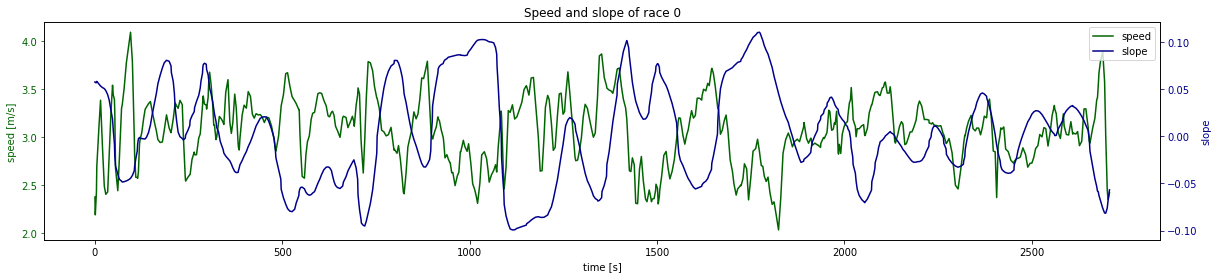
\includegraphics[width=\textwidth]{03_plot_speed_slope.png}
  \end{center}
\end{frame}

%------------------------------------------------

\begin{frame}
  \begin{center}
    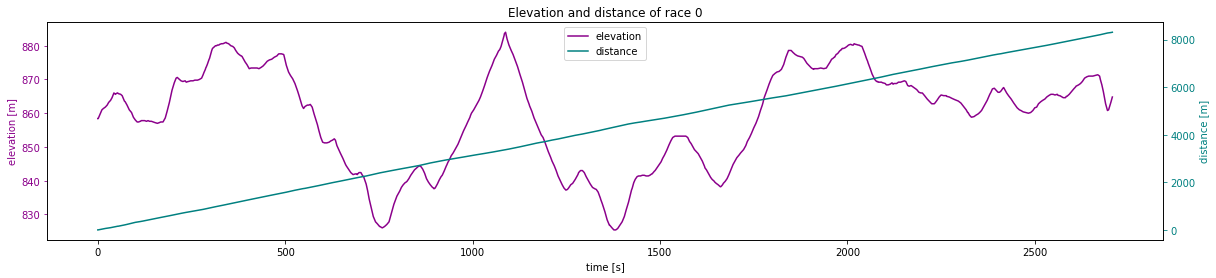
\includegraphics[width=\textwidth]{04_plot_elevation_distance.png}
  \end{center}
\end{frame}

%----------------------------------------------------------------------------------------
\section{Feature extraction}
%------------------------------------------------

\begin{frame}{Feature extraction}
	\begin{itemize}
    	\item \textbf{Features available}: distance, speed, elevation, time
		\item \textbf{Slope}: the slope is calculated with the distance and the elevation between points
        \item \textbf{Normalization}: min-max scaling
        \item \textbf{10 points to predict the 11$^{\text{th}}$}
	\end{itemize}
\end{frame}


%----------------------------------------------------------------------------------------
\section{Model}
%------------------------------------------------

\begin{frame}{LSTM}
	\begin{itemize}
    	\item Recurrent Neural Network without the vanishing gradient issue
        \item Composed of input gate, forget gate, output gate and memory cell
        \item \textit{adam} as optimizer
        \item Mean-Squared Error (MSE) as loss function
    \end{itemize}
\end{frame}

%----------------------------------------------------------------------------------------
\section{Results}
%------------------------------------------------
{\nologo
\begin{frame}{Results}
  \begin{table}[h]
    \begin{center}
      \begin{tabular}{|l||c|c|}
      \hline
      \textbf{Experiment} & \textbf{loss} & \textbf{val\_loss}\\
      \hline
      \hline
      A=feat.time-elevation-distance-speed-slope & 0.0603 & 0.0280\\
      B=feat.time-distance-speed-slope & 0.0591 & 0.0281\\
      C=feat.time-speed-slope & 0.0587 & \textbf{0.0278}\\
      D=feat.distance-speed-slope & 0.0551 & 0.0318\\
      E=feat.speed-slope & 0.0593 & 0.0287\\
      \textbf{F=feat.time-speed-slope-slopeNext} & 0.0589 & \textbf{0.0271}\\
      G=feat.time-speed-slope-slopeNext-avg5 & 0.0837 & 0.0519\\
      H=feat.time-speed-slope-slopeNext-batch1 & 0.0575  & 0.0345\\
      I=feat.time-speed-slope-slopeNext-batch100 & 0.1017 & 0.0455\\
      J=feat.time-speed-slope-slopeNext-units8 & \textbf{0.0532} & \textbf{0.0278}\\
      K=feat.time-speed-slope-slopeNext-units16 & 0.0415 & 0.0306\\
      L=feat.time-speed-slope-slopeNext-units32 & \textbf{0.0391} & 0.0322\\
      \hline
      \end{tabular}
    \end{center}
  \end{table}
\end{frame}
}

%------------------------------------------------

\begin{frame}
  \begin{center}
    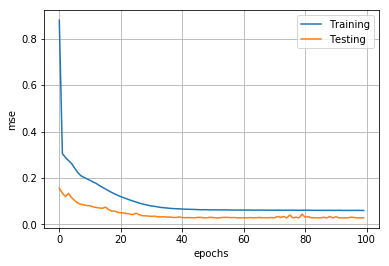
\includegraphics[scale=0.7]{01_score_feat_time_speed_slope_slopeNext.png}
  \end{center}
\end{frame}

%------------------------------------------------

\begin{frame}
  \begin{center}
    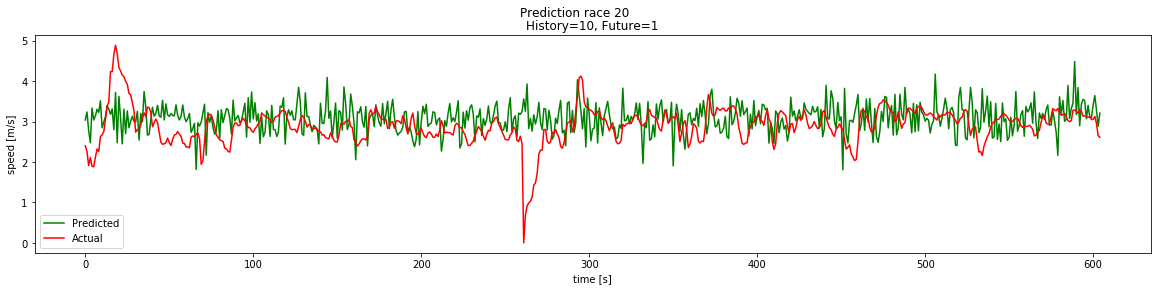
\includegraphics[width=\textwidth]{02_plot_feat_time_speed_slope_slopeNext.png}
  \end{center}
\end{frame}

%----------------------------------------------------------------------------------------
\section{Conclusion}
%------------------------------------------------

\begin{frame}{Conclusion}
    \begin{itemize}
        \item Predicted runs not close but with few resemblances
        \item More complex model with more data might improve
    \end{itemize}
\end{frame}

%----------------------------------------------------------------------------------------
\end{document}
